\bframe{Discrete}
\begin{equation*}
\dot{\mathbf{y}} = \mathbf{K}(t) \mathbf{y}
\end{equation*}

\begin{itemize}
\item Start with ortogonal vectors $\mathbf{y}^k$
\item Iterate
\item ``Gramm-Schmidt'' $\mathbf{y}^k$ and accumulate change
\end{itemize}
\eframe

\bframe{Discrete}
\begin{center}
  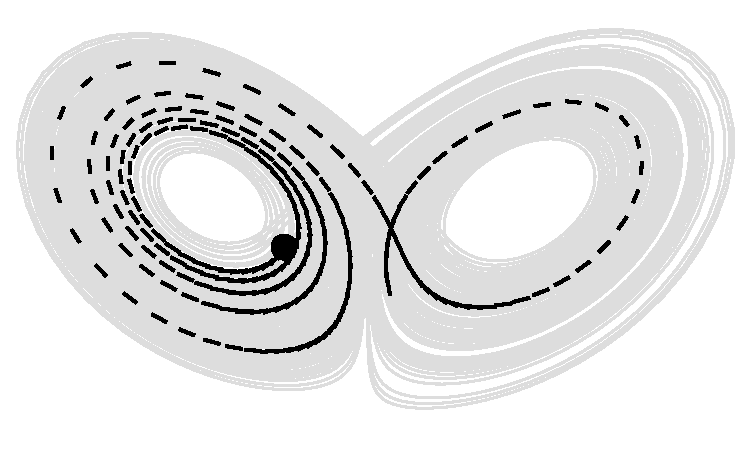
\includegraphics[width=\textwidth]{i/wolf.pdf}
\end{center}
\eframe

\bframe{Continues}
\begin{equation*}
\dot{\mathbf{y}} = \mathbf{K} \mathbf{y}, \quad
\dot{\mathbf{Y}} = \mathbf{K} \mathbf{Y}
\end{equation*}

\begin{equation*}
\mathbf{Y} = \mathbf{Q} \mathbf{R}
\end{equation*}

\begin{equation*}
\dot{\mathbf{Q}} = \text{RHS}(t, \mathbf{Q}),
\quad
\dot{\mathbf{R}} = \text{RHS}(t, \mathbf{R})
\end{equation*}

\eframe
